\documentclass[a4paper,11pt]{jsarticle}
\usepackage{amsmath,amssymb}
\usepackage{bm}
\usepackage[dvipdfmx]{graphicx}
\usepackage{here}

%テキストの表示領域の調節
\setlength{\textwidth}{\paperwidth}
\addtolength{\textwidth}{-40truemm}
\setlength{\textheight}{\paperheight}
\addtolength{\textheight}{-45truemm}

%余白の調節
\setlength{\topmargin}{-10.4truemm}
\setlength{\evensidemargin}{-5.4truemm}
\setlength{\oddsidemargin}{-5.4truemm}
\setlength{\headheight}{17pt}
\setlength{\headsep}{10mm}
\addtolength{\headsep}{-17pt}
\setlength{\footskip}{5mm}

\begin{document}

\section{課題A}時定数は(1)式のように導出することもできるが, 実機に対するパラメータ推定では
(1)式を用いた時定数推定は適切な値を導出できない. この理由を以下の1.1から1.3の手順に沿って確認する.

\begin{align}
		\tau=\frac{-T_d}{log(1-\frac{\dot{x}(T_d)}{Ak})}
\end{align}

\subsection{}
$T_d = 0.1〜1.0$の時の時定数を(1)式を用いて求め, $T_d$との関係をグラフにした(図1).この時$\dot{x}(T_d)$は,
実験で導出した$k=1.2370,\tau=0.02455,A=3$を用いて(2)式から求めた.
\begin{align}
		Ak(1-e^{-\frac{t}{\tau}})
\end{align}
\begin{table}[H]
	\caption{各Tdにおける時定数の値}
	\label{No.1}
	\begin{center}
		\begin{tabular}{|c|c|c|}\hline
			$T_d$ & $\dot{x}(T_d)$	& $\tau$ \\ \hline
			0.1	& 3.647695577	& 0.02455 \\ \hline
			0.2	& 3.709782237	& 0.02455 \\ \hline
			0.3	& 3.710839001	& 0.02455 \\ \hline
			0.4	& 3.710856988	& 0.02455 \\ \hline
			0.5	& 3.710857294	& 0.02455 \\ \hline
			0.6	& 3.710857299	& 0.02454999976 \\ \hline
			0.7	& 3.710857299	& 0.0245502868 \\ \hline
			0.8	& 3.710857299	& 0.02454464631 \\ \hline
			0.9	& 3.710857299	& 0.02449859503 \\ \hline
			1	& 3.710857299	& - \\ \hline
		\end{tabular}
\end{center}
\end{table}

\begin{figure}[H]
	\begin{center}
		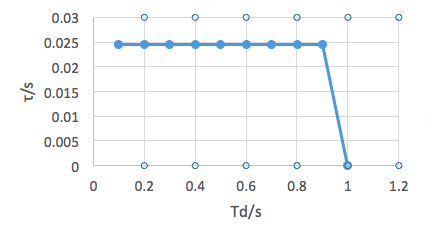
\includegraphics[width=10cm]{各Tdにおける時定数のグラフ.png}
		\caption{各Tdにおける時定数のグラフ}
		\label{各Tdにおける時定数のグラフ}
	\end{center}
\end{figure}


\subsection{}
図1を見ると$T_d=0.8$から小さくなり始め, $T_d=1$以降では急激に減少し$0$になることがわかる.
これは(1)式中の対数の真数が負になってしまうことにより, 値が計算できないことに起因している.
そこで, この真数の部分が1以上であるときの不等式を解いてみると以下のようになる.
\begin{align}
	\dot{x}(T_d)<Ak
\end{align}
すなわち$\dot{x}(T_d)<3.710857299$であれば(1)式は値を取ることができる. $T_d=0.9$及び$T_d=1$の時の$\dot{x}(T_d)$と一致しているため, 小数点第9位以降でこの値を超してしまったと思われる.
次に, $T_d$の変化によって$\tau$が変化してしまった理由について考察する.
実測から求めた時定数を$\tau'$として(2)式を(1)式に代入すると次のようになる.
\begin{align}
	\tau=\frac{-T_d}{log(e^{\frac{-T_d}{\tau'}})}=\tau'
\end{align}
つまり, 本来ならば$T_d$に依らず, 実測値との誤差は生まれないはずであることがわかる.
これは(2)式において一度指数計算を行ってから(1)式においてまた対数計算を行うという過程で(1)式の分母にのみわずかに誤差を生じたため, $T_d$の値が時定数の変化を生んだと考えられる.

\subsection{}
速度の計測誤差の影響を考察する. まず$T_d=0.1,A=3$として実測データを用い, (2)式から$\dot{x}(T_d)$を求めた.
その次に, 計測された速度を$\dot{x}(T_d)+\delta$とした時, $\delta=0〜0.1[m/s]$と時の$\tau$の値を(1)式によって求めた.
この時の値とグラフをそれぞれ表2と図2にまとめた.

\begin{table}[H]
	\caption{各速度誤差$\delta$における時定数$\tau$の値}
	\label{No.1}
	\begin{center}
		\begin{tabular}{|c|c|}\hline
			$\delta$ & $\tau$ \\ \hline
			0 & 0.02455 \\ \hline
			0.01 & 0.023553355 \\ \hline
			0.02 & 0.022451405 \\ \hline
			0.03 & 0.02119712 \\ \hline
			0.04 & 0.019698544 \\ \hline
			0.05 & 0.017725137 \\ \hline
			0.06 & 0.014148471 \\ \hline
			0.07 & - \\ \hline
			0.08 & - \\ \hline
			0.09 & - \\ \hline
			0.1 & - \\ \hline
		\end{tabular}
\end{center}
\end{table}

\begin{figure}[H]
	\begin{center}
		\includegraphics[width=10cm]{各速度誤差δにおける時定数のグラフ.png}
		\caption{各速度誤差$\delta$における時定数$\tau$のグラフ}
		\label{各速度誤差δにおける時定数のグラフ}
	\end{center}
\end{figure}
$\delta$が大きくなるにつれ, 時定数は減少していき, 1.1で求めた$T_d=0.1$における$\tau$との誤差が広がっていった.
(1)式の$T_d$が大きくなると分母の絶対値が大きくなっていくためである.\\
$\delta=0.06〜0.07$を境に(1)式の計算値が求められなくなっているが, 1.2で求めた不等式を考慮すると
\begin{align}
	T_d+0.06<3.710857299<T_d+0.07
\end{align}
となる事からも予測できる.

\section{課題B}
\subsection{}
比例制御とPI制御で制御された台車系の応答の変化を観察し, それぞれの制御の利点と問題点を考察する.
時間経過と台車の位置の関係を表したグラフが次の図3である.
\begin{figure}[H]
	\begin{center}
		\includegraphics[width=10cm]{PとPI比較1.bmp}
		\caption{台車系の応答}
		\label{台車系の応答}
	\end{center}
\end{figure}
まず外乱がない場合について考察する. この時P制御は0.35[s]ほどで第一目標位置に到達し,安定しているのに対し,
PI制御では6回ほどオーバーシュートしたのち, 約1.5[s]かかり第二目標地点に到達している. 第二目標地点についても同様に,
P制御がPI制御に比べ, すぐに目標地点に到達している. 次に外乱がない場合について考察する. P制御では定常偏差分だけ目標地点から
ずれたところに停止してしまっている. PI制御では数回のオーバーシュートがあるものの, 二回とも正確に目標地点に到達している.
以上の結果から, 外乱無しの場合にはP制御, 外乱ありの場合にはPI制御を用いることが適していると考えられる.
また, 目標位置に対して定常偏差以上に許容しても要件を満たす場合にはP制御で十分であるので, 要求される精度や使用する場面に
応じてどの制御を用いるかは柔軟に対応する必要があると考えられる.
\section{課題C}
\subsection{}
LQ制御の重み$q_1$の値に応じた台車の位置, 振り子の角度, 制御入力の値の違いを表したグラフを次の図4,5,6に示す.
\begin{figure}[H]
	\begin{center}
		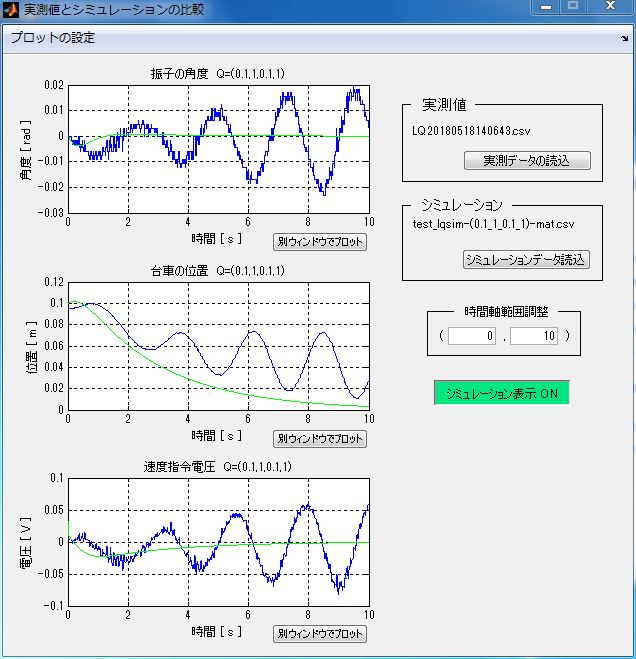
\includegraphics[width=8cm]{比較1.jpg}
		\caption{$q_1=0$の場合}
		\label{$q_1=0$の場合}
	\end{center}
\end{figure}

\begin{figure}[H]
	\begin{center}
		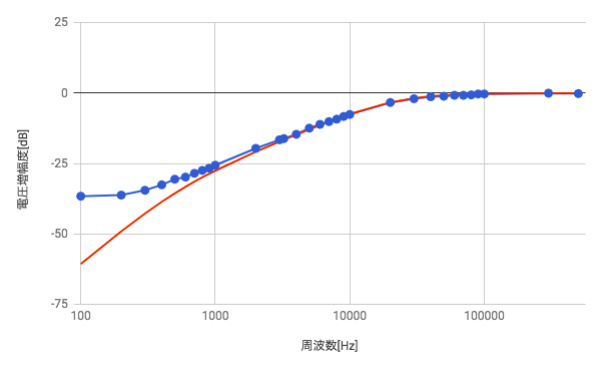
\includegraphics[width=8cm]{比較2.jpg}
		\caption{$q_1=1$の場合}
		\label{$q_1=1$の場合}
	\end{center}
\end{figure}

\begin{figure}[H]
	\begin{center}
		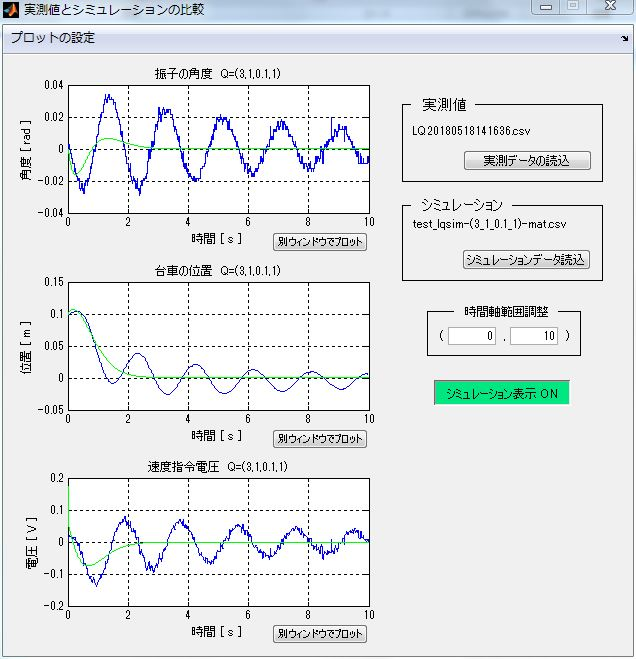
\includegraphics[width=8cm]{比較3.jpg}
		\caption{$q_1=3$の場合}
		\label{$q_1=3$の場合}
	\end{center}
\end{figure}

台車の位置についてグラフを比較する. $q_1$が大きくなるにつれ, 緑色の目標値と台車の位置の差分
の面積が小さくなっていることがわかる.  振り子の角度については$q_1=0$の時の振幅の最大値がおおよそ0.02[rad]
であり$q_1=1,q_1=3$の時には0.025[rad], 0.03[rad]と大きくなり, 目標値との差分の面積が大きくなっている.
つまり$q_1$を大きくすると台車の位置の精度は高くなるが振り子の角度の振れは大きくなってしまう.
これらの考察を評価関数とともに説明していく.今回の実験の制御で用いた評価関数は(6)式のように表すことができる.
\begin{align}
	\int^{\infty}_{0}q_1x^2(t)+q_2\theta^2(t)+q_3\dot{x}^2(t)+q_4\dot{\theta}^2(t)+u^2(t)dt
\end{align}
この式を最小化することで, それぞれのパラメータの和を最小化させることを目的としている.
例えば$q_1$を大きくすることで$x(t)$をより早く0に近づけようとするのである.
そのため, $q_1$が大きくなるにつれ上記のように台車の位置のオーバーシュートが小さくなるのである.
しかしながら依然としてオーバーシュートが残っている. この理由として, 今回用いた倒立振子モデルでは三角関数を
近似して運動方程式を線形化したことであるためと思われる.


\section{課題D}
回転のみにのみ自由度を持つ振子の制御を考える. $\theta$は垂直上向きからの角度, $m$は振子の質量,
$l$は回転軸から重心までの長さ, $I$は重心周りの慣性モーメント, $u$は制御入力とし, 回転摩擦は無視できるとする.
この振子を倒立させるための制御則を以下の1.1, 1.2の手順で設計する.
\subsection{}
まず, 振子の運動エネルギー$T$を求める.
\begin{align}
	T=\frac{1}{2}l\theta^2+\frac{1}{2}m(l\dot{\theta})^2
\end{align}
次に回転軸中心を原点としたポテンシャルエネルギー$U$を求める.
\begin{align}
	U=mgl\cos\theta
\end{align}
ラグランジアン$L$は$L=T-U$であるから,
\begin{align}
	L=T-U=\frac{1}{2}I\dot{\theta}^2+\frac{1}{2}m(l\dot{\theta})^2-mgl\cos\theta
\end{align}
となる. したがってラグランジュの運動方程式は
\begin{align}
	\dfrac{d}{dt}\left(\dfrac {\partial L}{\partial \dot{\theta}}\right)-\frac{\partial L}{\partial \theta}=0
\end{align}
であるから, (9)式を$\theta,\dot{\theta}$でそれぞれ偏微分したものを代入すると, 振子の運動方程式は外力$u$を用いて次のようになる.
\begin{align}
	(I+ml^2)\ddot{\theta}-mgl\sin\theta=u
\end{align}
\subsection{}
前問の振子の運動方程式を線形化した方程式$\bm{\dot{x}}=A\bm{x}+B\bm{u}$を導出する. ただし, 状態変数を$\bm{x}=\left[\dot{\theta},\theta\right]^{\mathrm{T}}$とする.\\
(11)式を変形すると
\begin{align}
	\ddot{\theta}=\frac{mgl}{I+ml^2}\theta+\frac{1}{I+ml^2}u
\end{align}
のとなる. これを$\bm{\dot{x}}=A\bm{x}+B\bm{u}$と係数比較する.
\begin{align}
	\dot{x}=\left(
	\begin{array}{cc}
	0 & \frac{mgl}{I+ml^2} \\
	1 & 0
	\end{array}\right)x+\left(
	\begin{array}{c}
	\frac{1}{I+ml^2} \\
	0
	\end{array}\right)u
\end{align}
したがって, $A$と$B$は
\begin{align}
	A=\left(
	\begin{array}{cc}
	0 & \frac{mgl}{I+ml^2} \\
	1 & 0
	\end{array}\right),
	B=\left(
	\begin{array}{c}
	\frac{1}{I+ml^2} \\
	0
	\end{array}\right)
\end{align}
と求められた.

\subsection{}
$l=1,m=1,I=1,g=10$の振子に対して
\begin{align}
	Q=\left[
	\begin{array}{cc}
		0 & 0 \\
		0 & 1
	\end{array}
	\right]
	R=1
\end{align}
の最適制御入力を求める.

1.2の結果に$l=1,m=1,I=1,g=10$を代入すると
\begin{align}
	A=\left(
	\begin{array}{cc}
	0 & 5 \\
	1 & 0
	\end{array}\right),
	B=\left(
	\begin{array}{c}
	\frac{1}{2} \\
	0
	\end{array}\right)
\end{align}
となる. $A,B,Q,R$を以下に示すリカッチ代数方程式に代入し, Pを求める.
\begin{align}
	A^{\mathrm{T}}P+PA-PBR^{-1}B^{\mathrm{T}}P+Q
\end{align}

\begin{align}
	P=\left[
	\begin{array}{cc}
		4\sqrt{10+\sqrt{101}} & 20+2\sqrt{101} \\
		20+2\sqrt{101} & 2\sqrt{101+10\sqrt{101}}
	\end{array}
	\right]
\end{align}
求められたPから最適制御入力を求めると
\begin{align}
	u=-R^{-1}B^{\mathrm{T}}P\bm{x}
\end{align}

\begin{align}
	u=-\left[
	\begin{array}{cc}
		2\sqrt{10+\sqrt{101}} & 10+\sqrt{101}
	\end{array}
	\right]\left[
	\begin{array}{c}
		\dot{\theta} \\
		\theta
	\end{array}
	\right]
\end{align}
となった.


\end{document}
